\chapter{GT-TİPİ YENİDEN YAPILANDIRILABİLİR ENERJİ DEPOLAMA MİMARİSİ}
\label{chap:gttipi}

Önceki bölümlerde üç seviyeli T-tipi dönüştürücünün düşük güç davranışı, ters akım dolaşımı, nötr anahtar susturma yöntemi, Sin\textsuperscript{3} tabanlı ileri besleme kompanzasyonu ve mevcut deney düzeneği incelenmiştir. Düşük güç incelemesi, anma gücü tasarım hedefi \SI{20}{\kilo\volt\ampere}--\SI{25}{\kilo\watt} olan evirici altyapısına ve erişilebilen düşük güç kayıtlarına dayanmaktadır. GT-tipi mimari ise aynı deney düzeneğinin doğrudan büyütülmüş sürümü değildir; proje başvuru formunda tanımlanan \SI{100}{\kilo\watt} hedefli, değiştirilmiş T-tipi güç katı ile aktif batarya yönetimini bir araya getiren ayrı bir tasarım katmanıdır \citep{Arifoglu2023Basvuru}. İki katman birbirinin yerine geçmez: T-tipi evirici, ölçüm, koruma ve düşük güç anahtarlama birikimi Bölüm~\ref{chap:sistem}--\ref{chap:deney} içinde korunmuş; GT-tipi mimari, şebeke arayüzü, izole şarj kolları, batarya bazlı kontrol ve yeniden yapılandırılabilir deşarj dizisini aynı sistem sınırında ilişkilendiren sonraki tasarım katmanı olarak ayrılmıştır.

``GT-tipi'' adı, tezde \emph{geliştirilmiş/değiştirilmiş T-tipi} enerji depolama mimarisini belirtmek için kullanılan proje içi bir adlandırmadır; literatürde standartlaşmış bağımsız bir çok seviyeli dönüştürücü ailesi değildir. Mimari; T-tipi/PFC şebeke katı, SiC tabanlı yüksek frekanslı köprü, çok sekonderli yalıtım transformatörleri, batarya başına DA/DA şarj kolları ve seçilebilir seri deşarj yolundan oluşan bütünleşik öneriyi ifade etmektedir.

Bölüm boyunca tasarım hedefi, doğrulanmış parametre ve deney sonucu birbirinden ayrılmıştır. Başvuru formundaki topoloji ve sayısal değerler ``proje hedefi'', Bölüm~\ref{chap:deney} altındaki kayıtlar ``prototip kanıtı'', literatür karşılaştırmaları ise ``dış kaynak kanıtı'' statüsündedir. \SI{100}{\kilo\watt} prototipin üretildiği veya belirtilen kiplerde deneysel olarak doğrulandığı yönünde bir sonuç iddiası kurulmamaktadır.

\section{Tasarım Gereksinimleri}
\label{sec:gt-gereksinimler}

Yüksek güçlü bir EDS'de batarya dizisi sabit ve ideal bir DA kaynak değildir. Hücre veya modül uç gerilimleri şarj durumu, sıcaklık, iç direnç, akım ve yaşlanmayla değişir; seri dizinin kullanılabilir kapasitesi zayıf birim tarafından sınırlandırılabilir \citep{Plett2015,Hannan2017,Farakhor2023}. Yeniden yapılandırılabilir batarya sistemleri, seçilen modülleri enerji yoluna alma veya yoldan çıkarma olanağıyla arıza yalıtımı, gerilim uyarlama ve kapasite kullanımını iyileştirmeyi hedefler \citep{Momayyezan2016,Farakhor2023,Huang2024}. İlave yarı iletkenler ise iletim kaybı, sürücü sayısı, koruma gereksinimi ve denetim karmaşıklığı oluşturduğundan tasarım değerlendirmesi yalnız işlev sayısına değil, kayıp ve güvenlik bedeline de dayanmalıdır.

Proje başvuru kaynağı; \SI{34.5}{\kilo\volt}/\SI{0.69}{\kilo\volt} şebeke transformatörü arkasında \SI{690}{\volt} fazlar arası gerilim, \SI{100}{\kilo\watt} toplam güç ve \SI{1000}{\volt} DA bara kontrol referansı öngörmektedir \citep{Arifoglu2023Basvuru}. Aynı kaynak, üç adet AB--BC--CA fazlar arası konteyner, konteyner başına dokuz şarj/deşarj alt birimi, yirmi bataryayı besleyen çok sekonderli yalıtım transformatörü ve batarya başına ölçüm/buck/bypass işlevleri tanımlamaktadır. Değerlerin ölçülmüş prototip parametresi olmadığı vurgulanmalıdır; Tablo~\ref{tab:gt-tasarim-gereksinimleri} gereksinimleri kanıt durumlarıyla birlikte toplamaktadır.

\begin{table}[htbp]
  \centering
  \caption{GT-tipi mimari için proje kaynağından çıkarılan tasarım gereksinimleri ve kanıt durumu \citep{Arifoglu2023Basvuru}.}
  \label{tab:gt-tasarim-gereksinimleri}
  \small
  \begin{tabularx}{\textwidth}{@{}p{0.24\textwidth}p{0.27\textwidth}X@{}}
    \toprule
    Gereksinim & Proje hedefi / aday değer & Tezdeki kullanım ve doğrulama gereksinimi \\
    \midrule
    Şebeke bağlantısı & \SI{34.5}{\kilo\volt}/\SI{0.69}{\kilo\volt} transformatör, \SI{690}{\volt} fazlar arası & Tasarım sınırı; gerçek transformatör etiketi, bağlantı grubu, kısa devre empedansı ve topraklama düzeni bekleniyor. \\
    Toplam güç & \SI{100}{\kilo\watt} & Proje hedefi; \SI{20}{\kilo\volt\ampere}--\SI{25}{\kilo\watt} tasarım hedefli T-tipi prototipin anma değeriyle birleştirilmez. \\
    DA bara & \SI{1000}{\volt} kontrol referansı & Başvuru şemasındaki aday referans; toplam/yarım bara, tolerans ve aşırı gerilim sınırı doğrulanacak. \\
    Şebeke katı & Üç seviyeli değiştirilmiş T-tipi, PFC, EMI ve LCL filtre & Doğrultma işlevi için öneri; yarı iletken, diyot, filtre ve denetleyici değerleri bekleniyor. \\
    Yüksek frekans katı & Altı SiC MOSFET, \SI{30}{\kilo\hertz}, üç fazlar arası transformatör grubu & Kaynak tasarım değeri; rezonans ağı, ölü zaman, sürme sırası ve manyetik tasarım doğrulanacak. \\
    Batarya şarjı & Çok sekonderli yalıtım ve batarya başına buck kolu & Her batarya için akım/gerilim kontrolü hedefi; sargı sayısı, izolasyon seviyesi ve buck değerleri bekleniyor. \\
    Deşarj yolu & Seçilebilir seri batarya yolu, paralel bypass diyodu, yedek batarya & Kademeli DA yük üzerinde sınanması öngörülüyor; şebekeye evirme proje test kapsamı dışında. \\
    Batarya izleme & Batarya başına gerilim, akım ve sıcaklık & Algılayıcı, örnekleme, doğruluk, haberleşme ve hata eşikleri bekleniyor. \\
    Güvenlik & Ön şarj, ark önleme, arıza yalıtımı, termal ve elektriksel sınırlar & IEC~62619, IEC~62477-1 ve IEC~62933-5-2 kapsamlarıyla ayrıntılı tehlike analizi yapılacak \citep{IEC62619,IEC62477,IEC62933_5_2}. \\
    \bottomrule
  \end{tabularx}
\end{table}

Tablo~\ref{tab:gt-tasarim-gereksinimleri}, aynı belgede geçen \SI{690}{\volt}, \SI{1000}{\volt}, \SI{30}{\kilo\hertz} ve \SI{100}{\kilo\watt} değerlerinin farklı fiziksel büyüklükler olduğunu görünür kılmaktadır. Bölüm~\ref{chap:sistem} altındaki \SI{431.5}{\volt} DA bara ve \SI{10}{\kilo\hertz} anahtarlama değerleri mevcut evirici/senaryo dosyalarına; Microchip kaynağındaki \SI{700}{\volt} ve \SI{140}{\kilo\hertz} değerleri harici Vienna PFC referans tasarımına aittir. Üç parametre kümesi tek bir modelin ayarları olarak kullanılamaz.

Tasarım gereksinimleri altı işlevsel ilkeye indirgenmiştir: enerji yolunun çift yönlü olabilmesi, şarj sırasında şebeke akım kalitesinin gözetilmesi, batarya kollarının galvanik olarak ayrılması, her bataryanın güvenli akım--gerilim--sıcaklık sınırlarında tutulması, arızalı/zayıf birimin seri yolu kesmeden bypass edilebilmesi ve her mod geçişinin ölçüm geri bildirimiyle güvenli biçimde tamamlanması. IEC~62619 endüstriyel ve sabit uygulamalardaki ikincil lityum hücre ve bataryaların güvenli işletimine; IEC~62477-1 güç elektroniği dönüştürücülerindeki elektrik çarpması, yangın, ısıl ve enerji tehlikelerine; IEC~62933-5-2 ise şebeke ile bütünleşik elektrokimyasal EDS'nin yaşam döngüsü boyunca alt sistem etkileşimlerinden doğan güvenlik risklerine odaklanmaktadır \citep{IEC62619,IEC62477,IEC62933_5_2}.

\section{GT-Tipi Topolojinin Yapısı}
\label{sec:gt-yapi}

GT-tipi kavramının gelişimi iki ayrı tasarım katmanına sahiptir. İlk katman, mevcut T-tipi faz kolunu RL1 fonksiyon anahtarıyla evirici, iki seviyeli transformatör besleme katı ve Vienna PFC işlevleri arasında yeniden görevlendirmektedir. İkinci katman, aynı işlev paylaşımı fikrini \SI{100}{\kilo\watt} hedefli AB--BC--CA konteynerleri, SiC köprüler ve batarya bazlı izole şarj kollarıyla genişleten proje mimarisidir. İki katman aşağıda ayrı alt başlıklarda verilmektedir.

\subsection{İlk Tasarım Katmanı: RL1 Tabanlı İşlev Paylaşımı}

T-tipi faz kolunun temel yapısı Bölüm~\ref{chap:sistem} içindeki Şekil~\ref{fig:t-tipi-uc-seviye} ve Şekil~\ref{fig:t-tipi-akim-yollari} ile verildiğinden burada yeniden basılmamıştır. İlk tasarım katmanının ayırt edici alt devreleri Şekil~\ref{fig:gt-viyana-pfc}--\ref{fig:gt-pfc-modu} üzerinde sırasıyla açıklanmaktadır.

Şekil~\ref{fig:gt-viyana-pfc} üzerindeki Vienna doğrultucu; üç faz giriş endüktansları, altı doğrultma diyodu, nötr IGBT grubu ve bölünmüş DA baradan oluşmaktadır. Şarj yönünde şebekeden düşük harmonikli ve birim güç faktörüne yakın akım çekmek için Vienna katı kullanılmaktadır. Devre, \SI{100}{\kilo\watt} başvuru şemasındaki değiştirilmiş PFC katıyla aynı uygulama ayrıntılarına sahip kabul edilmemelidir.

\begin{figure}[htbp]
  \centering
  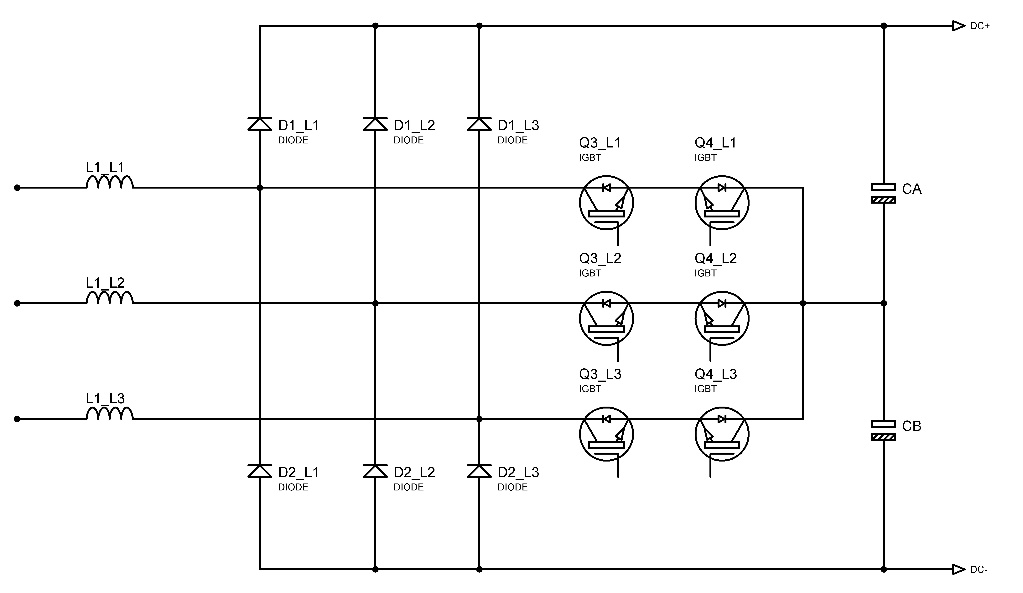
\includegraphics[width=0.92\textwidth]{gt-tipi/onceki_tez_6_2_viyana_pfc.jpeg}
  \caption{Vienna doğrultucu PFC devresi (ilk tasarım katmanı).}
  \label{fig:gt-viyana-pfc}
\end{figure}

Şekil~\ref{fig:gt-cok-sekonderli-bys}, tek primer ve çok sayıda sekonder sargı üzerinden her bataryaya ayrı doğrultucu--buck kolu sağlamaktadır. Her çıkışta diyot doğrultma, DA bağlantı kondansatörü, kontrollü anahtar, serbest dolaşım diyodu, endüktans ve çıkış kondansatörü bulunmaktadır. Batarya bazında şarj akımı ve gerilimi ayarlama hedefi sekonder kollarının fiziksel ayrışmasına dayanmaktadır.

\begin{figure}[htbp]
  \centering
  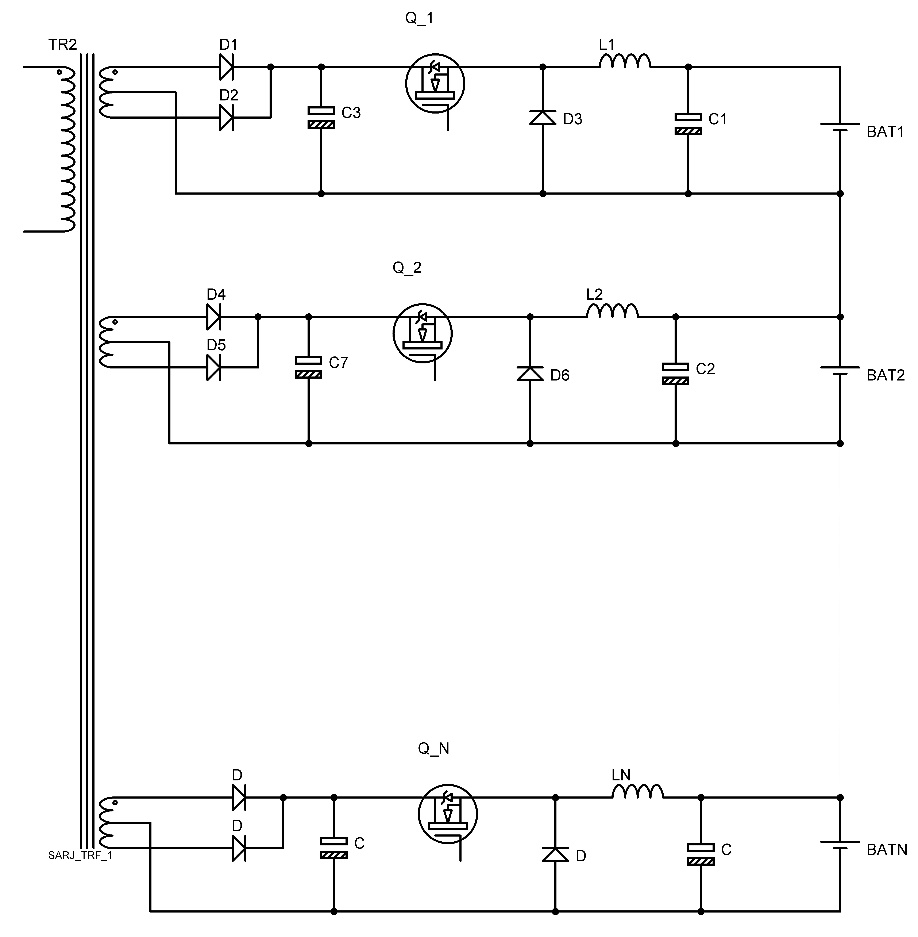
\includegraphics[width=0.67\textwidth]{gt-tipi/onceki_tez_6_3_cok_sekonderli_bys.jpeg}
  \caption{Tek primer ve çoklu sekonder sargılı transformatör içeren aktif BYS prensip devresi.}
  \label{fig:gt-cok-sekonderli-bys}
\end{figure}

Yaklaşımın ayırt edici bağlantısı Şekil~\ref{fig:gt-ana-topoloji} üzerinde görülmektedir. RL1, yarım köprü kolundaki $Q_1$--$Q_2$ anahtarları ile nötr kolundaki $Q_3$--$Q_4$ anahtarlarının ortak T-tipi çıkış düğümündeki işlevsel bağlantısını değiştirmektedir: bir konumda tam T-tipi evirici ve LCL filtre, diğer konumda iki seviyeli yüksek frekans katı ile ayrı PFC yolu oluşmaktadır.

\begin{figure}[htbp]
  \centering
  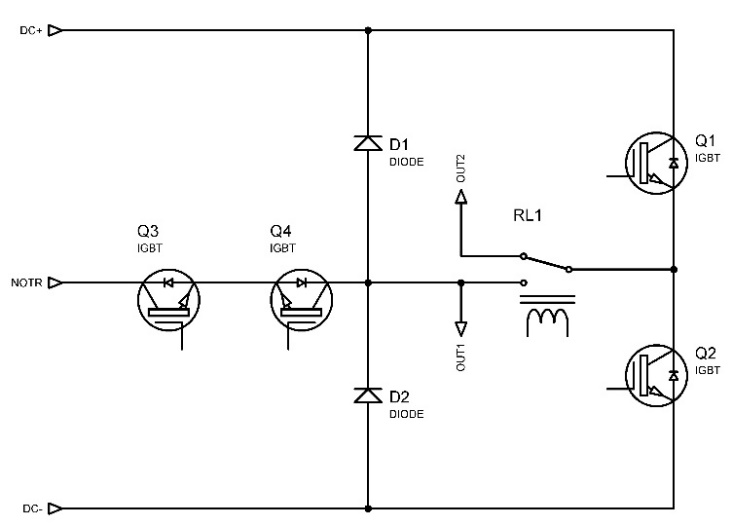
\includegraphics[width=0.82\textwidth]{gt-tipi/onceki_tez_6_4_gt_tipi_ana_topoloji.jpeg}
  \caption{GT-tipi ana topoloji ve RL1 fonksiyon anahtarı.}
  \label{fig:gt-ana-topoloji}
\end{figure}

RL1 ve RL2'nin evirici konumundaki bağlantısı Şekil~\ref{fig:gt-evirici-lcl} üzerinde gösterilmiştir. $Q_1$--$Q_4$ grubu bölünmüş DA bara ile faz çıkışı arasında üç seviyeli T-tipi kolu oluşturmakta; $L_1$--$C$--$L_2$ ağı şebeke akımını filtrelemektedir. Görsel, deşarj yönündeki temel güç yolunu açıklamaktadır; şebekeye deşarjın \SI{100}{\kilo\watt} prototip için gerçekleştirildiği anlamına gelmemektedir.

\begin{figure}[htbp]
  \centering
  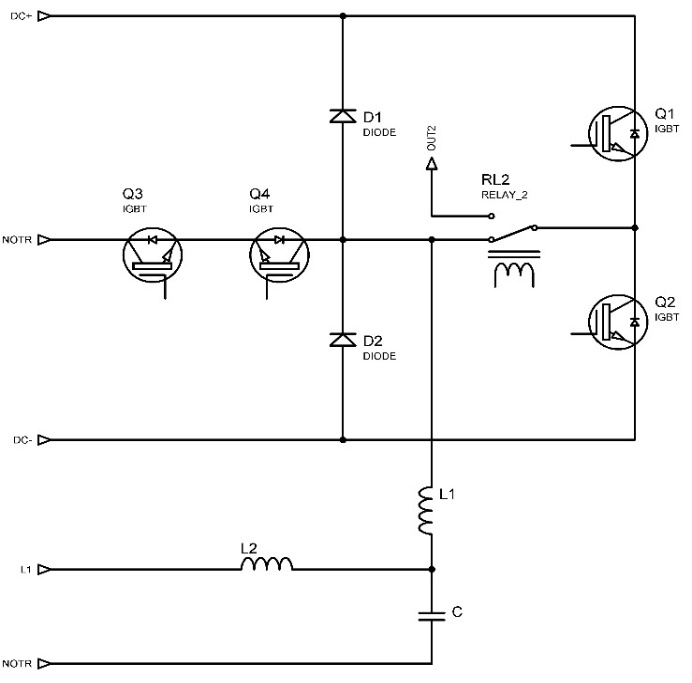
\includegraphics[width=0.76\textwidth]{gt-tipi/onceki_tez_6_5_evirici_lcl_modu.jpeg}
  \caption{GT-tipi topolojinin evirici çalışma modu ve LCL filtre bağlantısı.}
  \label{fig:gt-evirici-lcl}
\end{figure}

Şekil~\ref{fig:gt-iki-seviye-trafo}, üç fazın yarım köprü anahtarlarını üç adet çok sekonderli transformatörün primerleriyle ilişkilendirmektedir. Yalnız deşarjda kullanılan $Q_1$--$Q_2$ yarım köprülerinin şarj sırasında transformatör besleme katına dönüştürülmesi, yarı iletkenlerin atıl kalmasını önleyen birinci yeniden kullanım yoludur.

\begin{figure}[htbp]
  \centering
  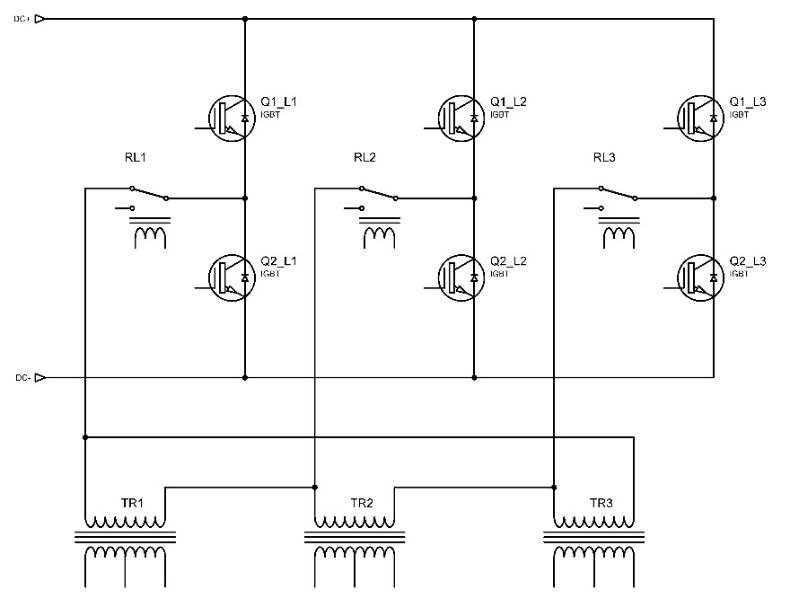
\includegraphics[width=0.88\textwidth]{gt-tipi/onceki_tez_6_6_iki_seviye_trafo_modu.jpeg}
  \caption{İki seviyeli evirici çıkışları ve çok sekonderli BYS transformatörleri.}
  \label{fig:gt-iki-seviye-trafo}
\end{figure}

İkinci yeniden kullanım yolu Şekil~\ref{fig:gt-pfc-modu} üzerinde verilmiştir: nötr IGBT çiftleri, doğrultma diyotları ve LCL elemanlarıyla üç fazlı Vienna PFC kollarına dönüştürülmektedir. Şekil~\ref{fig:gt-evirici-lcl}--\ref{fig:gt-pfc-modu} birlikte okunduğunda GT-tipi adının yalnız yeni bir devre çiziminden değil, aynı anahtar gruplarının enerji yönüne göre farklı görevlerde kullanılmasından kaynaklandığı görülmektedir.

\begin{figure}[htbp]
  \centering
  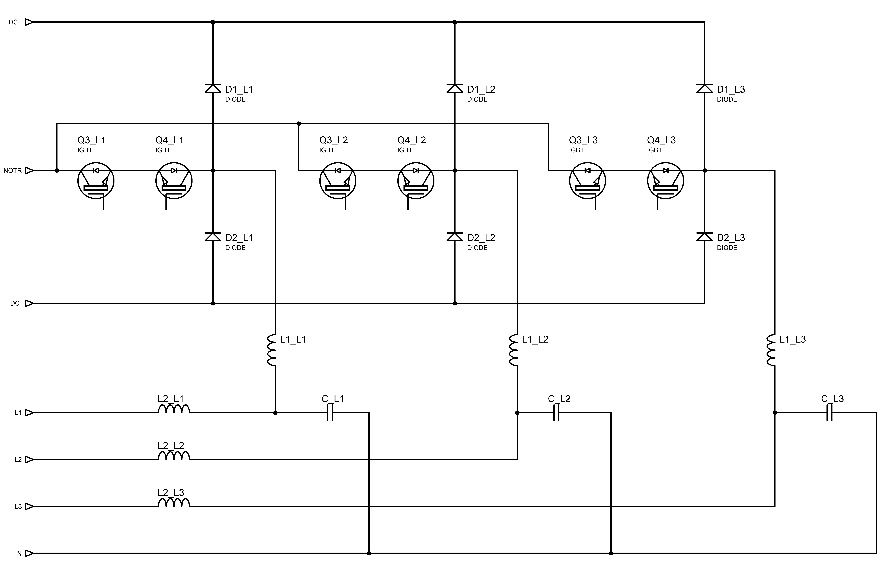
\includegraphics[width=0.94\textwidth]{gt-tipi/onceki_tez_6_7_pfc_modu.jpeg}
  \caption{Nötr IGBT gruplarıyla oluşturulan üç fazlı PFC bölümü.}
  \label{fig:gt-pfc-modu}
\end{figure}

\subsection{100 kW Hedefli Proje Mimarisi}

Şekil~\ref{fig:gt-basvuru-guc-kati}, proje başvuru formundaki değiştirilmiş T-tipi güç katını kaynağındaki işaretlerle korumaktadır. Şebeke tarafındaki transformatör, EMI filtresi ve LCL filtre sonrasında altı IGBT'li üç seviyeli PFC katı bulunmaktadır. Bölünmüş DA bara, diyot köprüleri ve altı SiC MOSFET'li yüksek frekanslı köprü, fazlar arasına bağlı transformatör gruplarını besleyecek biçimde gösterilmiştir. ``MOD'' işareti şarj ile deşarj yönündeki anahtarlama düzenini seçen üst seviye komutu temsil etmektedir. Şema kavramsal bağlantıyı gösterir; anahtar gerilim/akım değerleri, sürücü devreleri, ölü zamanlar, filtre elemanları ve koruma eşikleri verilmediğinden imalat şeması değildir.

\begin{figure}[htbp]
  \centering
  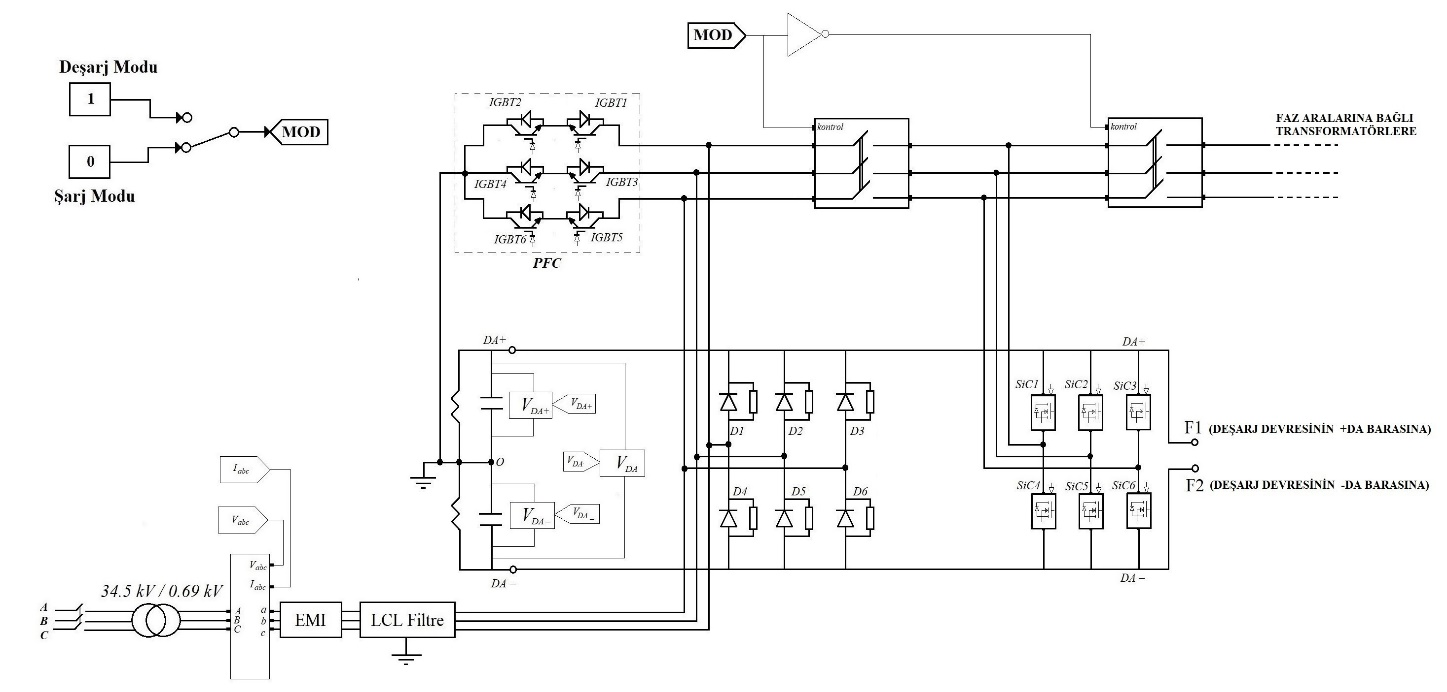
\includegraphics[width=0.98\textwidth]{gt-tipi/basvuru-degistirilmis-t-tipi-guc-kati.jpg}
  \caption{Proje başvuru kaynağındaki değiştirilmiş T-tipi, PFC özellikli güç katı ve fazlar arası transformatör çıkışları \citep{Arifoglu2023Basvuru}.}
  \label{fig:gt-basvuru-guc-kati}
\end{figure}

Sistem gücünün fazlar arası üç alt yapıya dengeli dağıtıldığı ideal durumda toplam güç referansı
\begin{equation}
  P_{\mathrm{GT}}^{\star}=P_{AB}^{\star}+P_{BC}^{\star}+P_{CA}^{\star},
  \qquad
  P_{AB}^{\star}\simeq P_{BC}^{\star}\simeq P_{CA}^{\star}\simeq
  \frac{P_{\mathrm{GT}}^{\star}}{3}
  \label{eq:gt-guc-paylasimi}
\end{equation}
biçiminde yazılabilir. Eşitlik~\eqref{eq:gt-guc-paylasimi} içinde $P_{\mathrm{GT}}^{\star}$ toplam hedef gücü; $P_{AB}^{\star}$, $P_{BC}^{\star}$ ve $P_{CA}^{\star}$ ilgili faz çifti konteynerlerinin güç referanslarını gösterir. \SI{100}{\kilo\watt} hedef için ideal dengeli pay yaklaşık \SI{33.3}{\kilo\watt} değerindedir; bölüşüm bir ölçüm sonucu değil, faz akımlarını dengeli tutmak için kullanılacak başlangıç tasarım koşuludur.

Şekil~\ref{fig:gt-basvuru-sarj-desarj}, AB konteyneri içinde çoğaltılan şarj/deşarj alt birimlerini, çok sekonderli yalıtım transformatörünü, batarya başına DA/DA kolunu ve seri deşarj yolunu birlikte göstermektedir; aynı yapı BC ve CA faz çiftleri için yinelenmektedir. Kaynak çizimde her konteynerde dokuz alt birim ve her alt birimde kırk sekonder çıkış üzerinden yirmi bataryaya ait iki kutuplu bağlantı gösterilmektedir. Sayıların nihai donanım yerleşimi sayılabilmesi için transformatör imalat dosyası, batarya konfigürasyonu ve kablolama listesi gereklidir.

\begin{figure}[htbp]
  \centering
  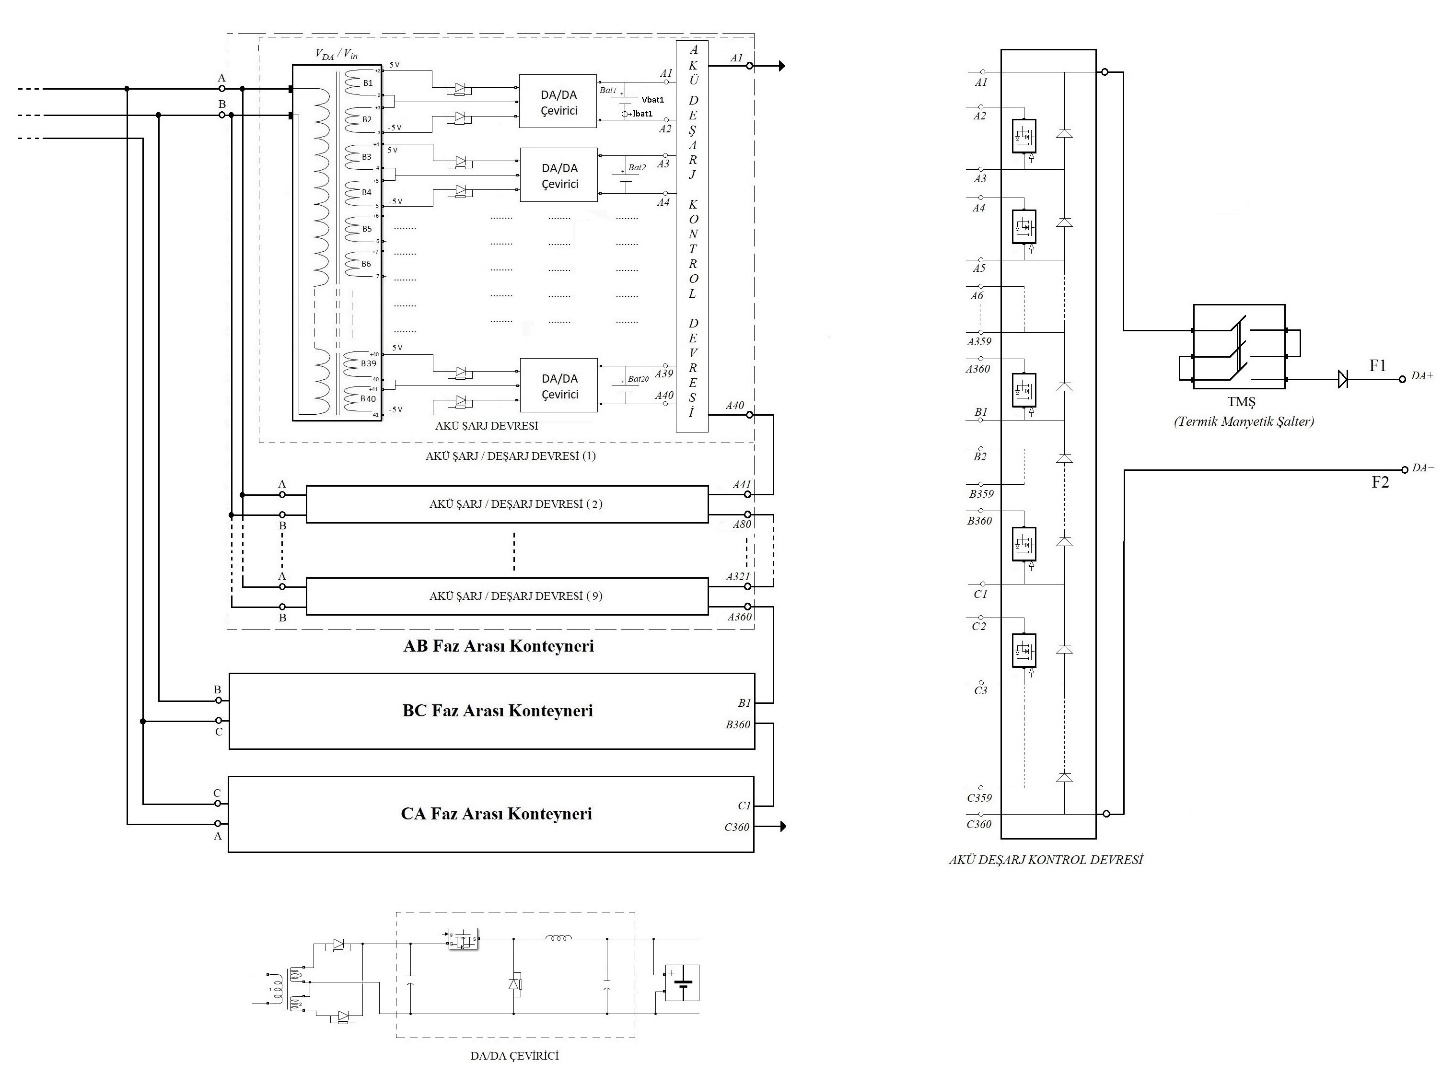
\includegraphics[width=0.96\textwidth]{gt-tipi/basvuru-sarj-desarj-konteyner-mimarisi.jpg}
  \caption{Proje başvuru kaynağındaki AB--BC--CA konteynerleri, izole şarj kolları ve seçilebilir seri deşarj yolu \citep{Arifoglu2023Basvuru}.}
  \label{fig:gt-basvuru-sarj-desarj}
\end{figure}

Batarya dizisindeki $N_b$ birimden hangilerinin seri deşarj yoluna alındığı $s_k\in\{0,1\}$ seçim değişkeniyle gösterildiğinde dizi geriliminin ideal bağıntısı
\begin{equation}
  v_{\mathrm{str}}(t)=\sum_{k=1}^{N_b}s_k(t)v_{b,k}(t)
  -\sum_{k=1}^{N_b}\bigl[1-s_k(t)\bigr]v_{D,k}(t)
  \label{eq:gt-dizi-gerilimi}
\end{equation}
olur. Eşitlik~\eqref{eq:gt-dizi-gerilimi} içinde $v_{\mathrm{str}}$ seri dizinin uç gerilimini, $v_{b,k}$ $k$ numaralı bataryanın uç gerilimini ve $v_{D,k}$ bypass yolundaki diyotun ileri yön gerilim düşümünü belirtmektedir; $s_k=1$ bataryanın seri yola alındığını, $s_k=0$ bypass edildiğini ifade eder. Gerçek devrede MOSFET iletim düşümü, kablo/bağlantı direnci ve anahtarlama geçişleri de eklenmelidir. Bağıntı, bypass edilen birim sayısı arttıkça DA bara gerilimi ile diyot kaybının birlikte değişeceğini açıklar.

Her bataryanın ayrı izole buck kolundan şarj edilmesi, seri deşarj bağlantısından farklı bir enerji yolu oluşturur. Şarj durumunda batarya akımları bağımsız ayarlanabilirken deşarj durumunda etkin birimlerden aynı dizi akımı geçer. İşlev ayrımı, ``batarya bazında dengeleme'' hedefinin şarj ve deşarj için aynı fiziksel mekanizmaya dayanmadığını gösterir: şarjda bağımsız akım/gerilim düzenleme, deşarjda birim seçimi ve bypass kullanılmaktadır.

\begin{figure}[htbp]
  \centering
  \begin{tikzpicture}[
    font=\small,
    block/.style={draw,rounded corners,align=center,minimum width=26mm,minimum height=12mm,fill=blue!5},
    batt/.style={draw,rounded corners,align=center,minimum width=26mm,minimum height=12mm,fill=green!8},
    ctrl/.style={draw,rounded corners,align=center,minimum width=29mm,minimum height=12mm,fill=orange!10},
    flow/.style={-{Latex[length=2.2mm]},thick},
    signal/.style={-{Latex[length=2mm]},dashed}
  ]
    \node[block] (grid) {\SI{690}{\volt} AA\\EMI + LCL};
    \node[block,right=9mm of grid] (pfc) {Değiştirilmiş\\T-tipi PFC};
    \node[block,right=9mm of pfc] (dc) {Bölünmüş\\DA bara};
    \node[block,right=9mm of dc] (sic) {SiC köprü\\\SI{30}{\kilo\hertz}};
    \node[block,below=12mm of sic] (tr) {AB--BC--CA\\yalıtım trafoları};
    \node[batt,left=9mm of tr] (buck) {Batarya başına\\izole buck};
    \node[batt,left=9mm of buck] (battery) {Batarya dizileri\\ve yedek birimler};
    \node[batt,below=12mm of battery] (load) {Seçilebilir seri yol\\ve kademeli DA yük};
    \node[ctrl,below=12mm of dc] (ems) {Üst seviye kip ve\\güç paylaşım denetimi};

    \draw[flow] (grid) -- node[above,font=\scriptsize]{şarj} (pfc);
    \draw[flow] (pfc) -- (dc);
    \draw[flow] (dc) -- (sic);
    \draw[flow] (sic) -- (tr);
    \draw[flow] (tr) -- (buck);
    \draw[flow] (buck) -- (battery);
    \draw[flow] (battery) -- node[left,font=\scriptsize]{deşarj} (load);
    \draw[signal] (ems) -- (pfc);
    \draw[signal] (ems) -- (sic);
    \draw[signal] (ems) -- (buck);
    \draw[signal] (ems) -- (battery);
  \end{tikzpicture}
  \caption{Kaynak şemalardan sentezlenen GT-tipi enerji ve denetim katmanları; oklar şarj ve kademeli yüke deşarj yönlerini göstermektedir.}
  \label{fig:gt-sentez-mimarisi}
\end{figure}

Şekil~\ref{fig:gt-sentez-mimarisi}, kaynak çizimlerde farklı sayfalara dağılan güç ve denetim katmanlarını tek bir işlevsel akışta birleştirmektedir. PFC katı şebeke akımı ile DA bara gerilimini, SiC köprü ve transformatör katı yalıtılmış enerji aktarımını, batarya başına buck kolları şarj akım/gerilimlerini, seri seçim ağı ise deşarj gerilimini belirler. Aynı anda bütün katların hızlı anahtarlanması gerekmez; batarya seçimi ve kip geçişleri, güç dönüştürücü PWM'inden daha yavaş bir üst seviye durum makinesiyle yönetilmelidir.

\section{Şarj Yönündeki Benzetim Kayıtları}
\label{sec:gt-benzetim}

GT-tipi topolojinin şarj yönündeki işlevsel bütünlüğü; Vienna PFC, iki seviyeli transformatör besleme katı ve batarya şarj kolunu aynı Simulink modeli içinde çalıştıran bir benzetimle gösterilmiştir. Şekil~\ref{fig:gt-simulink-modeli}--\ref{fig:gt-batarya-soc} yalnız sonuç grafikleri değildir; şebekeden bataryaya uzanan PFC $\rightarrow$ DA bara $\rightarrow$ transformatör primeri $\rightarrow$ sekonder $\rightarrow$ buck/batarya zincirinin her aşamasını belgelemektedir. Kaynak model dosyası ve ham zaman serileri mevcut olmadığı için kayıtlar bağımsız olarak yeniden hesaplanamamaktadır; kanıt statüleri nitel gösterim düzeyiyle sınırlandırılmıştır.

Şekil~\ref{fig:gt-simulink-modeli}; PFC denetimi, DA bara, üç fazlı dönüştürücü, çok sekonderli transformatörler ve batarya alt sistemlerinin aynı modelde kurulduğunu göstermektedir. Ekran görüntüsü blok adlarını ayrıntılı incelemek için yeterli çözünürlükte değildir; model hiyerarşisinin ve sonuç zincirinin varlığını belgelemek amacıyla verilmiştir.

\begin{figure}[htbp]
  \centering
  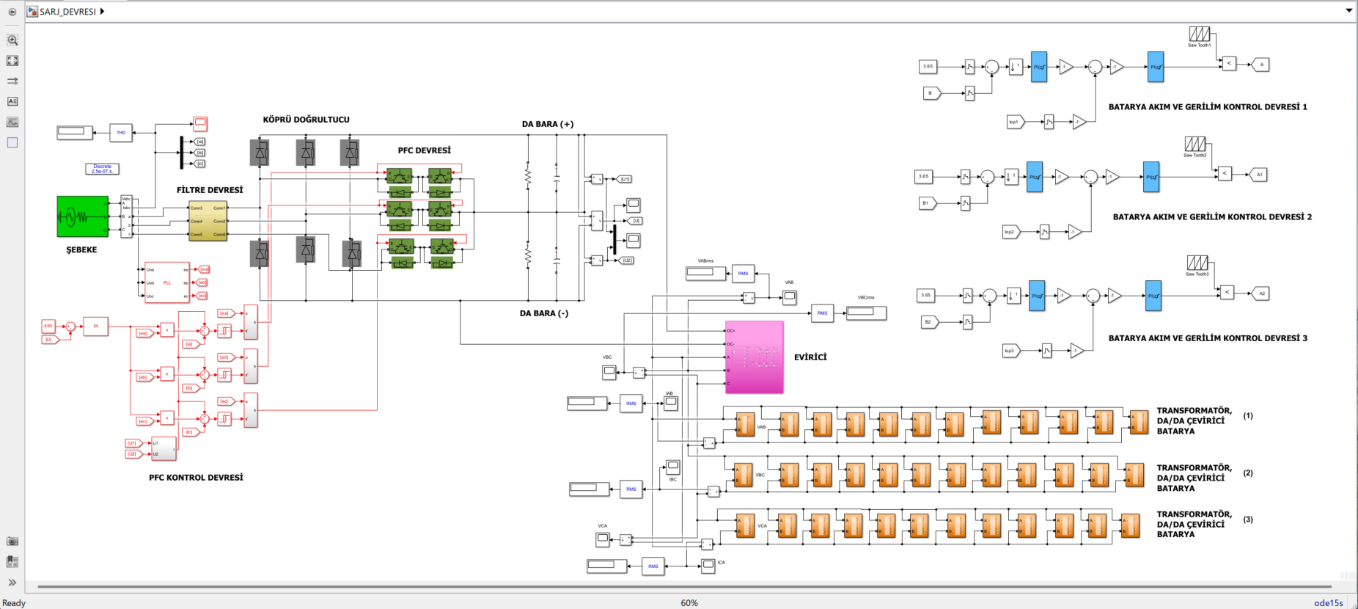
\includegraphics[width=0.98\textwidth]{gt-tipi/onceki_tez_6_8_simulink_modeli.png}
  \caption{Şarj yönündeki Vienna PFC, iki seviyeli evirici ve transformatör tabanlı BYS Simulink modeli.}
  \label{fig:gt-simulink-modeli}
\end{figure}

Şekil~\ref{fig:gt-pfc-akimlari}, PFC sonrasında üç faz akımının dengeli ve yaklaşık sinüzoidal biçimde oluştuğunu göstermektedir. Eksen birimleri, başlangıç koşulu, analiz penceresi, THD hesabı ve model parametreleri grafikten tek başına doğrulanamadığından görsel, PFC işlevinin çalıştığına ilişkin nitel kanıt olarak kullanılmıştır.

\begin{figure}[htbp]
  \centering
  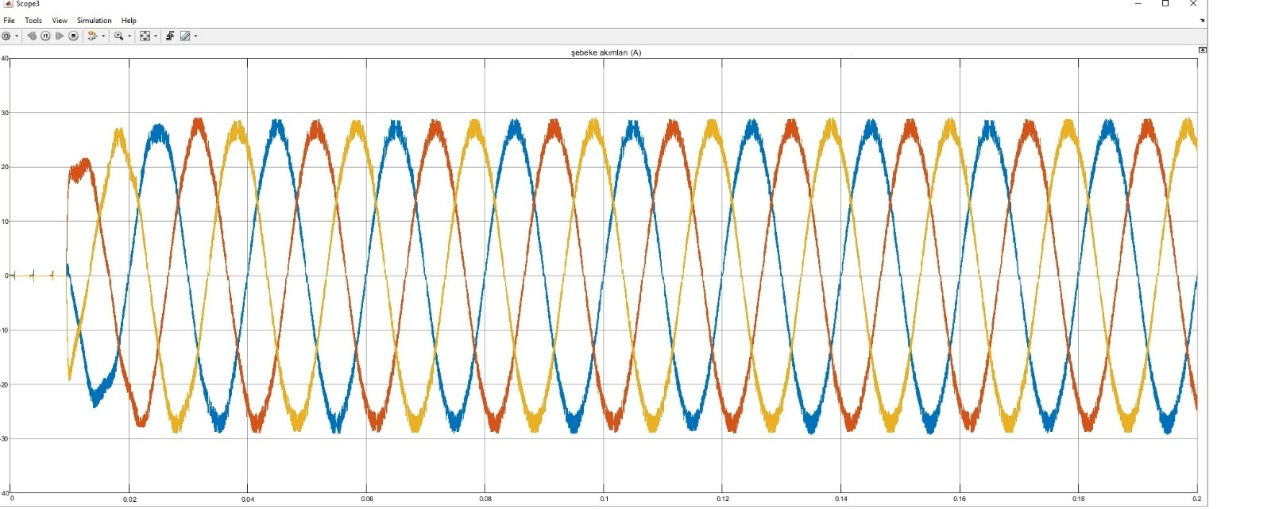
\includegraphics[width=0.96\textwidth]{gt-tipi/onceki_tez_6_9_pfc_sebeke_akimlari.jpeg}
  \caption{Vienna PFC sonrasındaki üç faz şebeke akımları.}
  \label{fig:gt-pfc-akimlari}
\end{figure}

Şekil~\ref{fig:gt-da-bara}, DA bara gerilimlerinin başlangıç geçicisinden sonra birbirine yakın bir çalışma bandına yerleştiğini göstermektedir. Referansın toplam bara mı, yarım bara mı olduğu ve düşey eksenin kesin değeri ham model olmadan kilitlenemediğinden grafik yalnız regülasyon davranışını nitel olarak destekler.

\begin{figure}[htbp]
  \centering
  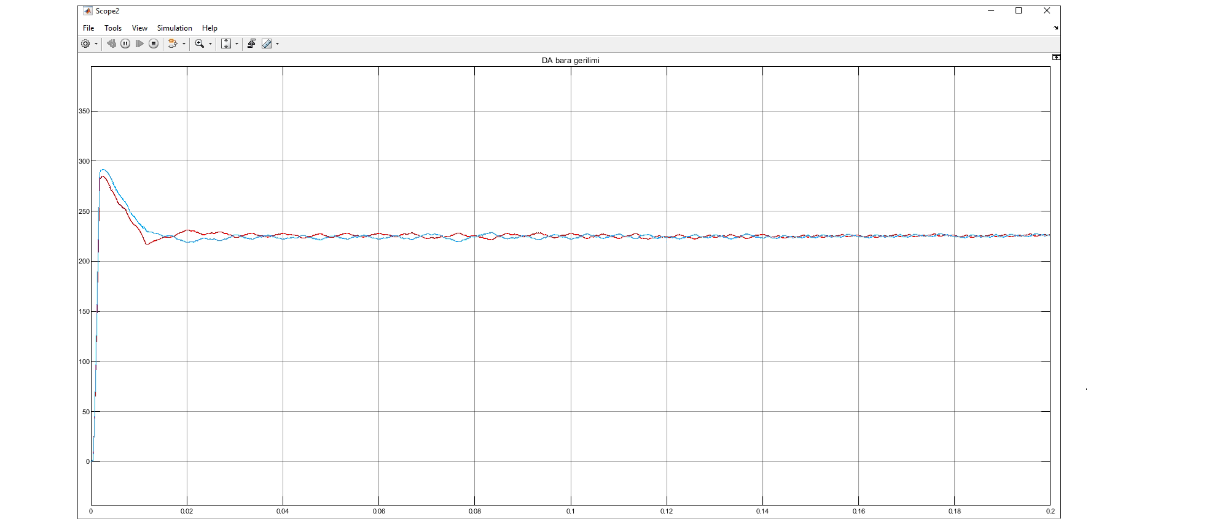
\includegraphics[width=0.96\textwidth]{gt-tipi/onceki_tez_6_10_da_bara_gerilimleri.png}
  \caption{DA bara gerilimlerinin zamanla değişimi.}
  \label{fig:gt-da-bara}
\end{figure}

İki seviyeli yüksek frekans katının transformatör primerine uyguladığı gerilim Şekil~\ref{fig:gt-primer-gerilim}, primer akımı Şekil~\ref{fig:gt-primer-akim} üzerindedir. Primer geriliminin pozitif, sıfır ve negatif seviyeler arasında değişmesi, görev oranı üzerinden transformatöre aktarılan gücün ayarlanabildiğini gösterir. Primer akımı aynı anahtarlama dizisine yanıt vermekte; kenarlardaki eğimler eşdeğer endüktans ve manyetik devre dinamiğinin etkisini göstermektedir. Sayısal kayıp veya transformatör verimi, sarım ve manyetik parametreler bulunmadan çıkarılmamıştır.

\begin{figure}[htbp]
  \centering
  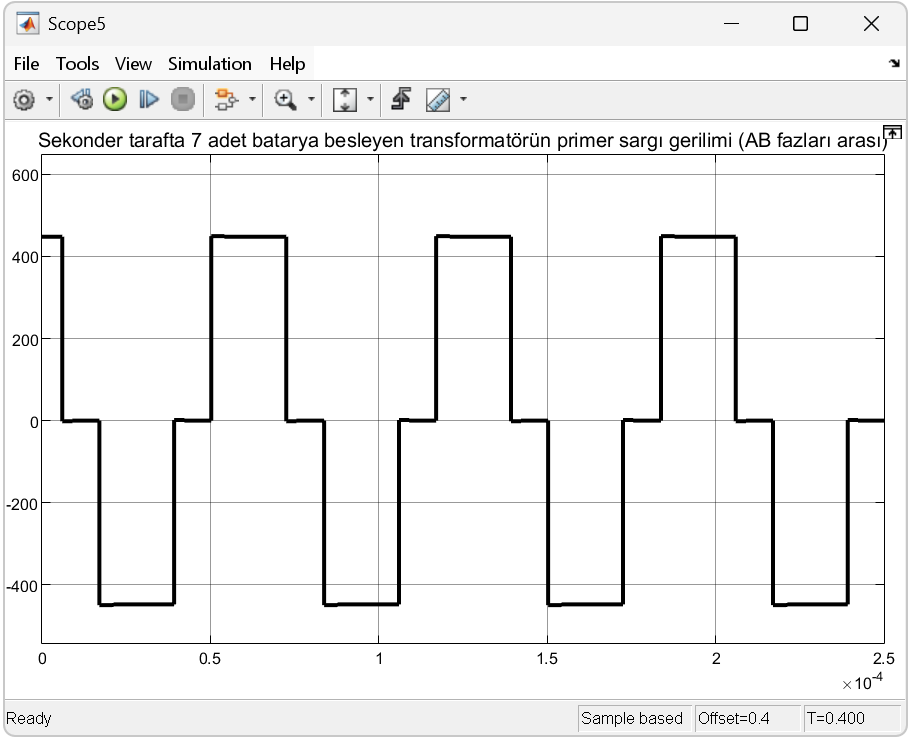
\includegraphics[width=0.76\textwidth]{gt-tipi/onceki_tez_6_11_primer_gerilim.png}
  \caption{BYS transformatörü primer sargı gerilimi.}
  \label{fig:gt-primer-gerilim}
\end{figure}

\begin{figure}[htbp]
  \centering
  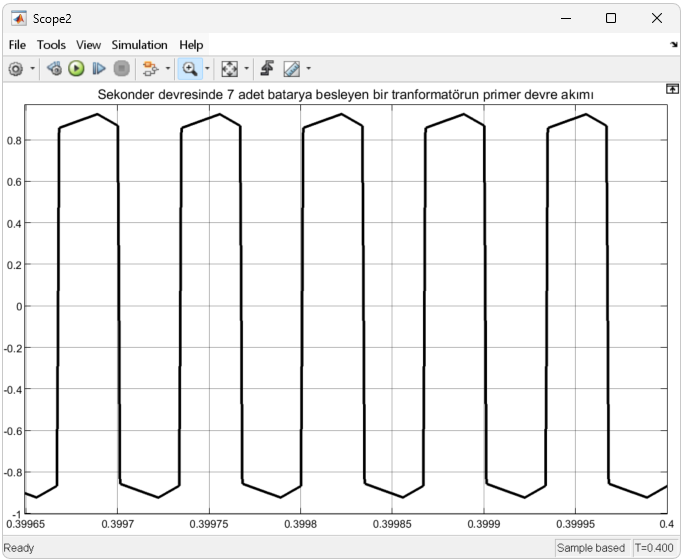
\includegraphics[width=0.76\textwidth]{gt-tipi/onceki_tez_6_12_primer_akim.png}
  \caption{BYS transformatörü primer akımı.}
  \label{fig:gt-primer-akim}
\end{figure}

Şekil~\ref{fig:gt-sekonder-gerilim} ve Şekil~\ref{fig:gt-sekonder-akim}, bir bataryayı besleyen sekonder sargının doğrultma öncesi gerilim ve akımını göstermektedir. Gerilim işaret değiştiren darbeli yapıya sahipken akımın pozitif enerji aktarım aralıklarında belirginleşmesi, sekonder doğrultucu ve buck girişinin primer anahtarlamasıyla eşzamanlı çalıştığını gösterir. Dönüş oranı, kaçak endüktans ve doğrultucu düşümleri bilinmediğinden primer--sekonder genlikleri üzerinden kesin verim hesabı yapılmamıştır.

\begin{figure}[htbp]
  \centering
  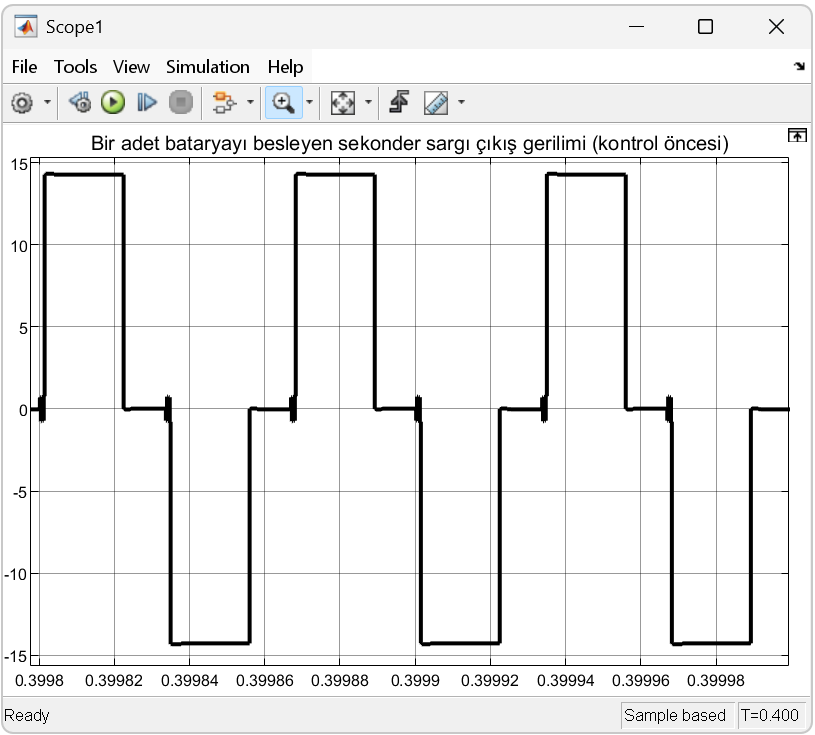
\includegraphics[width=0.76\textwidth]{gt-tipi/onceki_tez_6_13_sekonder_gerilim.png}
  \caption{BYS transformatörü sekonder sargı gerilimi.}
  \label{fig:gt-sekonder-gerilim}
\end{figure}

\begin{figure}[htbp]
  \centering
  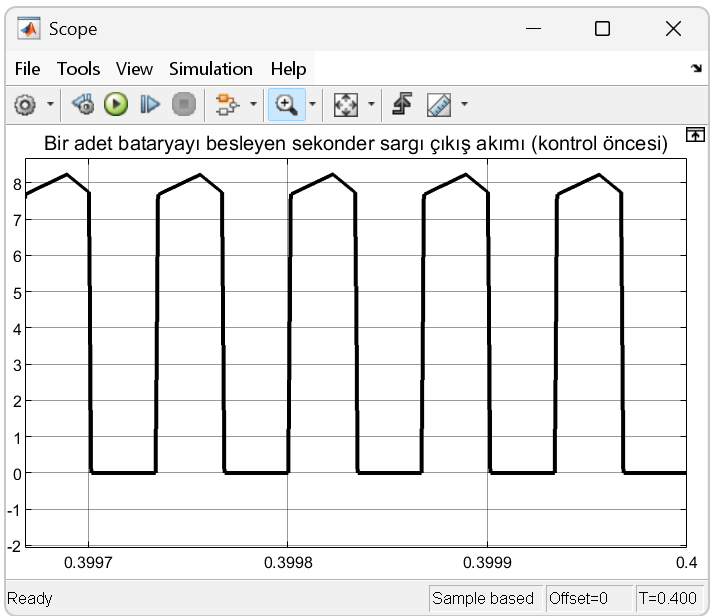
\includegraphics[width=0.76\textwidth]{gt-tipi/onceki_tez_6_14_sekonder_akim.png}
  \caption{BYS transformatörü sekonder sargı akımı.}
  \label{fig:gt-sekonder-akim}
\end{figure}

Enerji zincirinin batarya tarafındaki son kaydı Şekil~\ref{fig:gt-batarya-soc} üzerindedir; bir bataryanın şarj durumu (State of Charge, SoC), uç gerilimi ve akımı aynı zaman ekseninde verilmiştir. İşaret yönü ve ölçekler model değişken tanımlarına bağlı olduğundan değerler fiziksel deney sonucu olarak yorumlanmamıştır; kaydın görevi, PFC ve transformatör dalga biçimlerinin batarya durumuyla ilişkilendirildiğini göstermektir.

\begin{figure}[htbp]
  \centering
  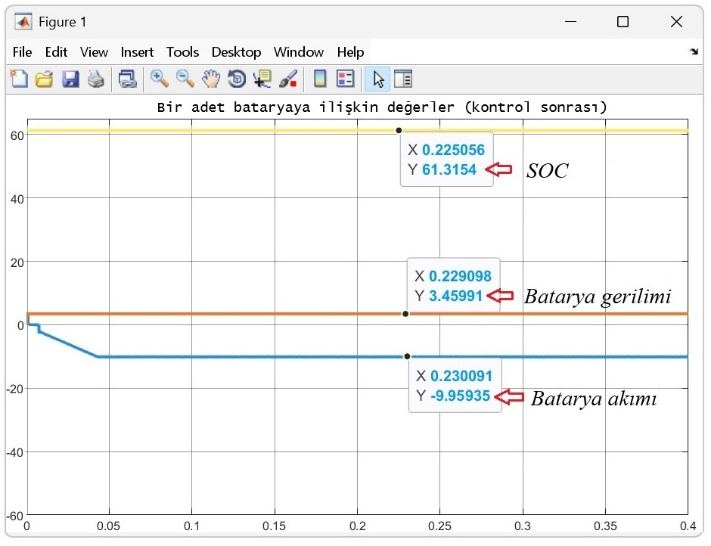
\includegraphics[width=0.80\textwidth]{gt-tipi/onceki_tez_6_15_batarya_soc.jpeg}
  \caption{Bir bataryaya ait SoC, uç gerilimi ve akım kayıtları.}
  \label{fig:gt-batarya-soc}
\end{figure}

Kayıtlar birlikte değerlendirildiğinde şarj yönündeki enerji aktarım zincirinin bütün alt basamakları temsil edilmektedir. Aynı kayıtlar; deşarj yönünde T-tipi evirici çalışmasını, RL1 geçişini, bypass/yedekleme davranışını, farklı güç seviyelerini veya deneysel performansı doğrulamamaktadır.

Şarj zinciri kayıtlarının yeniden üretilmesi için gereken kaynak model dosyası, çağrılan parametre dosyaları, çözücü ayarları, PFC ve DA bara referansları, anahtarlama frekansları ile transformatör ve batarya parametreleri tez kapsamında bulunmamaktadır. \SI{100}{\kilo\watt} katman için de güç kartı şeması, malzeme listesi (Bill of Materials, BOM), SiC, IGBT, MOSFET ve diyot parça kodları, çok sekonderli transformatörün sarım ve izolasyon bilgileri, batarya kimyası ve kapasitesi tanımlı değildir. Şekil~\ref{fig:gt-simulink-modeli}--\ref{fig:gt-batarya-soc} kayıtları ham zaman serisinden yeniden hesaplanamadığından THD, güç faktörü, verim ve SoC için sayısal sonuç verilmemekte; kayıtlar yalnız şarj zincirinin işlevsel bütünlüğüne ilişkin nitel gösterim olarak kullanılmaktadır. Sınırlılık açıktır: GT-tipi mimari için tezde yeniden üretilebilir benzetim kanıtı ve deney kanıtı yoktur; mimari, bir öneri ve gelecek çalışma konusu düzeyinde sunulmaktadır. Anahtarlamalı modelin kurulması ve ölçekli prototip deneyi, Bölüm~\ref{sec:gt-dogrulama} altındaki doğrulama matrisinin ilk adımları olarak gelecek çalışmaya bırakılmıştır.

\section{Şarj ve Deşarj Çalışma Modları}
\label{sec:gt-modlar}

GT-tipi yapının çalışması tek bir ``çift yönlü'' komutla açıklanamaz. Şebeke katı, yüksek frekans köprüsü, batarya buck kolları, seri seçim anahtarları, kontaktörler ve bypass yolları için izin verilen durumların birlikte tanımlanması gerekir. Tablo~\ref{tab:gt-calisma-modlari}, kaynak belgedeki işlevleri güvenli bir durum dizisine dönüştürmektedir.

\begin{table}[H]
  \centering
  \caption{GT-tipi mimarinin önerilen çalışma modları ve geçiş koşulları.}
  \label{tab:gt-calisma-modlari}
  \small
  \begin{tabularx}{\textwidth}{@{}p{0.18\textwidth}p{0.23\textwidth}X@{}}
    \toprule
    Mod & Etkin güç yolu & Temel koşul ve amaç \\
    \midrule
    Güvenli kapalı & Bütün PWM'ler ve ana kontaktörler kapalı & Enerjisiz başlatma, kilitli hata veya bakım durumu; artık gerilim denetlenir. \\
    Ön şarj / öz sınama & Sınırlı akımlı DA bara yolu ve ölçümler & İzolasyon, kontaktör geri bildirimi, sensör makullüğü ve DA bara gerilim yükselme hızı kontrol edilir. \\
    Şebekeden şarj & EMI--LCL--T-tipi PFC--DA bara--SiC köprü--trafo--buck--batarya & Şebeke akımı, DA bara, transformatör ve batarya sınırları birlikte korunur. \\
    CC şarj & Batarya başına buck akım düzenleme & Batarya üreticisinin akım ve sıcaklık sınırları içinde sabit akım uygulanır. \\
    CV şarj & Batarya başına buck gerilim düzenleme & Üst gerilim sınırında akım azalıncaya kadar sabit gerilim uygulanır. \\
    Kademeli yüke deşarj & Seçilen bataryalar--seri MOSFET yolu--DA yük & Şebekeye enerji verilmeden yük bankasına güç aktarılır; dizi gerilimi birim seçimiyle ayarlanır. \\
    Bypass / yedekleme & Zayıf birim devre dışı, bypass diyodu ve uygun yedek birim etkin & Gerilim, sıcaklık, SoC veya hata sınırını aşan birimin seri akım yolunu kesmeden ayrılması hedeflenir. \\
    Bakım/darbe modu & Yalnız uygun kimyadaki seçilmiş batarya ve buck kolu & Desülfasyon/hafıza etkisi işlemi genel EDS modu değildir; üretici sınırı, kimya ve deney protokolü doğrulanmadan etkinleştirilmez. \\
    \bottomrule
  \end{tabularx}
\end{table}

Batarya başına şarj referansı, CC--CV geçişini açıkça göstermek için
\begin{equation}
  i_{b,k}^{\star}=
  \begin{cases}
    I_{\mathrm{CC},k}, & v_{b,k}<V_{\mathrm{CV},k}\ \land\ T_{\min,k}<T_{b,k}<T_{\max,k},\\
    \operatorname{sat}\!\left[K_{v,k}\left(V_{\mathrm{CV},k}-v_{b,k}\right),0,I_{\mathrm{CC},k}\right],
      & v_{b,k}\geq V_{\mathrm{CV},k},\\
    0, & \text{koruma veya bypass koşulu}
  \end{cases}
  \label{eq:gt-cccv-referansi}
\end{equation}
biçiminde tanımlanabilir. Eşitlik~\eqref{eq:gt-cccv-referansi} içinde $i_{b,k}^{\star}$ $k$ numaralı bataryanın şarj akımı referansını, $I_{\mathrm{CC},k}$ sabit akım sınırını, $V_{\mathrm{CV},k}$ sabit gerilim eşiğini, $T_{b,k}$ ölçülen batarya sıcaklığını, $T_{\min,k}$ ve $T_{\max,k}$ izin verilen sıcaklık sınırlarını, $K_{v,k}$ gerilim düzenleyici kazancını ve $\operatorname{sat}[\cdot]$ doyum işlemini göstermektedir. Sayısal sınırlar batarya kimyası ve üretici veri sayfasından alınmadan atanmayacaktır.

Coulomb sayımına dayalı ayrık zamanlı şarj durumu güncellemesi
\begin{equation}
  \operatorname{SoC}_k[n+1]=\operatorname{sat}\!\left[
  \operatorname{SoC}_k[n]+\frac{\eta_{c,k}i_{b,k}[n]T_s}{Q_{n,k}},\,0,\,1\right]
  \label{eq:gt-soc-guncelleme}
\end{equation}
olarak yazılmıştır \citep{Plett2015}. Eşitlik~\eqref{eq:gt-soc-guncelleme} içinde $\operatorname{SoC}_k[n]$ $n$ örnekleme anındaki şarj durumunu, $\eta_{c,k}$ Coulomb verimini, $i_{b,k}[n]$ işaretli batarya akımını, $T_s$ BYS örnekleme süresini ve $Q_{n,k}$ güncel kullanılabilir kapasiteyi belirtmektedir; akım işareti şarj yönünde pozitif seçilmiştir. Akım sensörü ofseti ve kapasite yaşlanması nedeniyle yalnız Coulomb sayımı uzun süreli kullanımda sürüklenebilir; başlangıç düzeltmesi ve periyodik kestirim güncellemesi ayrıca tanımlanmalıdır.

Şekil~\ref{fig:gt-basvuru-tetikleme}, başvuru kaynağında DA bara/PFC denetimi ile SiC köprü darbe düzenini aynı görselde vermektedir. Üst kısımda \SI{1000}{\volt} DA bara referansı, PLL tabanlı faz bilgisi ve IGBT kapı komutları; alt kısımda \SI{30}{\kilo\hertz} temel dizilim ve görev oranı $d$ ile kısaltılan SiC darbeleri gösterilmiştir. Kaynak çizim; denetleyici katsayılarını, örnekleme sürelerini, ölü zamanı, doyumları ve koruma önceliğini eksiksiz vermediğinden gerçek zamanlı kodun yerine kullanılamaz.

\begin{figure}[H]
  \centering
  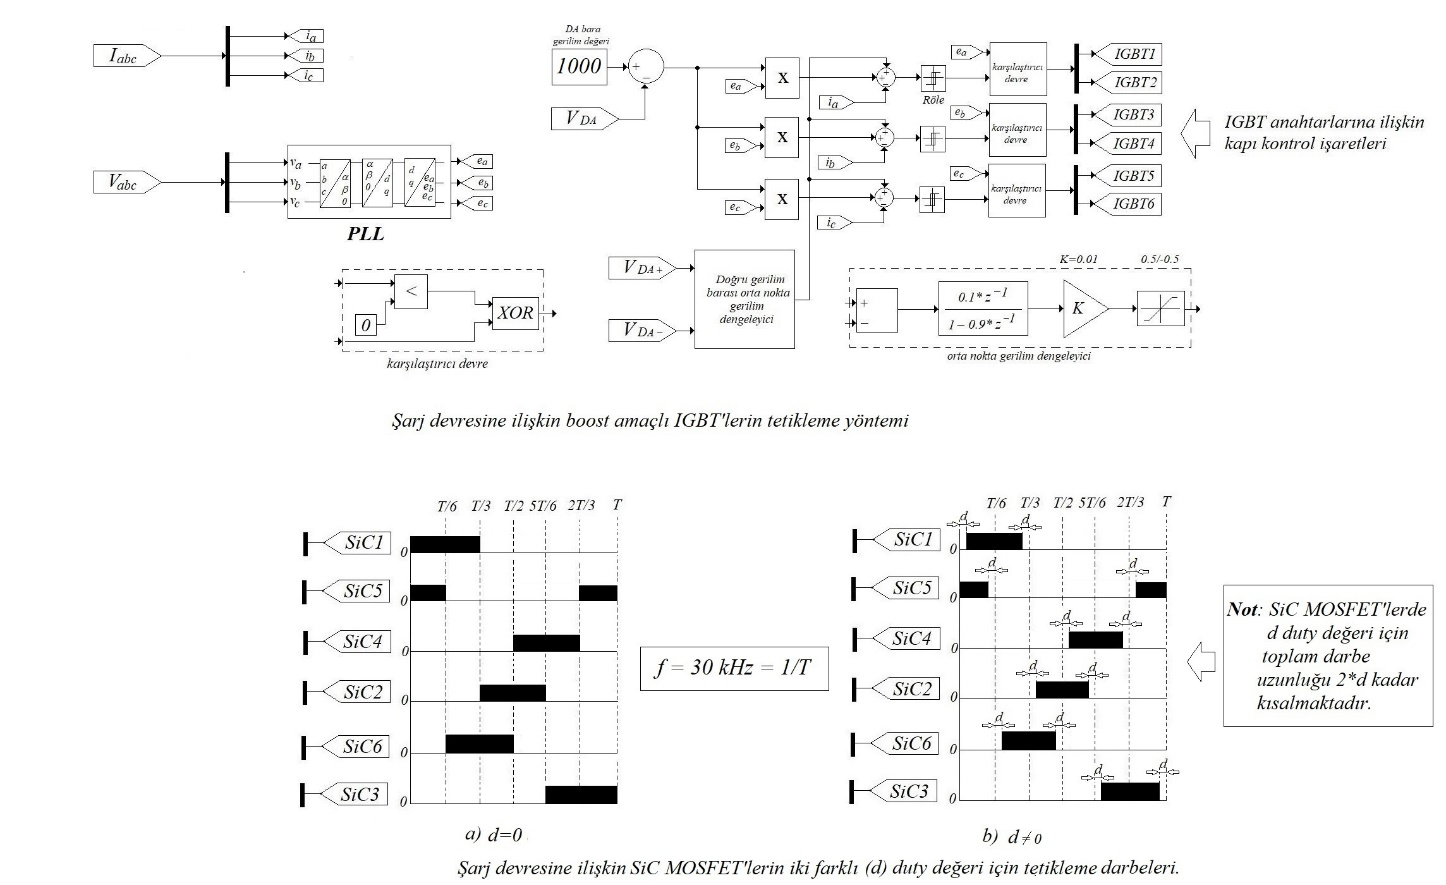
\includegraphics[width=0.96\textwidth]{gt-tipi/basvuru-igbt-sic-tetikleme.jpg}
  \caption{Proje başvuru kaynağındaki IGBT PFC denetimi ve iki farklı görev oranı için SiC MOSFET tetikleme düzeni \citep{Arifoglu2023Basvuru}.}
  \label{fig:gt-basvuru-tetikleme}
\end{figure}

Şekil~\ref{fig:gt-basvuru-tetikleme} içindeki IGBT eşlemeleri, PLL işaretleri, karşılaştırıcı mantığı, nötr nokta dengelemesi, SiC sırası, görev oranı tanımı, ölü zaman ve PWM güncelleme anı gerçek kontrol kodu ya da kesin bir Simulink modeliyle doğrulanmamıştır; tetikleme düzeni tezde nitel bir denetim mimarisi olarak sunulmaktadır. Başvuru metnindeki \SI{3}{\kilo\hertz} desülfasyon ifadesinin buck çıkış referans darbesine mi yoksa anahtarlama frekansına mı ait olduğu kaynak belgeden belirlenememektedir; ifade sayısal tasarım değeri olarak kullanılmamıştır. Desülfasyon, yalnız uygun kurşun-asit ya da NiCd kimyası ve üretici sınırları için geçerli bir bakım kipi olarak ele alınmakta, lityum iyon bataryalara genellenmemektedir. Gömülü yazılımın gerçeklenmesi ve tetikleme mantığının donanım üzerinde doğrulanması gelecek çalışma kapsamındadır.

\section{Mod Geçişleri ve Güvenlik Kısıtları}
\label{sec:gt-gecis-guvenlik}

Yeniden yapılandırma sırasında iki farklı gerilimdeki batarya veya bara düğümünün doğrudan birleştirilmesi, sınırlanmamış dengeleme akımına ve arka neden olabilir. Seri seçim ağı için \emph{önce kes--sonra bağla} ilkesi, sıfıra yakın dizi akımı ve düğüm gerilimi eşleşmesi birlikte aranmalıdır. Önerilen izin koşulu
\begin{equation}
  \gamma_{k\rightarrow j}=1
  \iff
  |i_{\mathrm{str}}|\leq I_{\mathrm{tr}}
  \ \land\
  |v_{\mathrm{node},k}-v_{\mathrm{node},j}|\leq \Delta V_{\mathrm{tr}}
  \ \land\
  h_k=h_j=1
  \label{eq:gt-gecis-izni}
\end{equation}
şeklinde ifade edilmiştir. Eşitlik~\eqref{eq:gt-gecis-izni} içinde $\gamma_{k\rightarrow j}$ $k$ durumundan $j$ durumuna geçiş iznini, $i_{\mathrm{str}}$ seri dizi akımını, $I_{\mathrm{tr}}$ geçiş için izin verilen akım eşiğini, $v_{\mathrm{node},k}$ ve $v_{\mathrm{node},j}$ bağlanacak düğümlerin gerilimlerini, $\Delta V_{\mathrm{tr}}$ izin verilen gerilim farkını ve $h_k,h_j$ ilgili kontaktör/anahtar geri bildirimlerinin sağlıklı olduğunu gösterir. Sayısal eşikler yarı iletken güvenli çalışma alanı, bağlantı endüktansı, ön şarj direnci ve ölçüm belirsizliğiyle belirlenmelidir.

\begin{figure}[htbp]
  \centering
  \begin{tikzpicture}[
    scale=0.95,
    transform shape,
    node distance=9mm and 13mm,
    state/.style={draw,rounded corners,align=center,minimum width=27mm,minimum height=10mm,fill=blue!5,font=\small},
    safe/.style={state,fill=green!10},
    fault/.style={state,fill=red!8},
    arr/.style={-{Latex[length=2mm]},thick},
    guard/.style={font=\scriptsize,align=center}
  ]
    \node[safe] (off) {Güvenli kapalı};
    \node[state,right=of off] (pre) {Ön şarj ve\\öz sınama};
    \node[state,right=of pre] (ready) {Hazır};
    \node[state,below left=of ready] (charge) {Şarj\\PFC + CC/CV};
    \node[state,below right=of ready] (dis) {Deşarj\\kademeli yük};
    \node[state,below=of ready] (reconf) {Bypass /\\yeniden yapılandırma};
    \node[fault,below=19mm of reconf] (fault) {Kilitli hata};

    \draw[arr] (off) -- node[above,guard]{başlat} (pre);
    \draw[arr] (pre) -- node[above,guard]{ölçüm ve\\geri bildirim uygun} (ready);
    \draw[arr] (ready) -- node[left,guard]{şarj izni} (charge);
    \draw[arr] (ready) -- node[right,guard]{yük hazır} (dis);
    \draw[arr] (charge) -- node[above,guard]{akım sıfıra yakın} (reconf);
    \draw[arr] (dis) -- node[above,guard]{akım sıfıra yakın} (reconf);
    \draw[arr] (reconf) -- node[right,guard]{gerilim eşleşti} (ready);
    \draw[arr] (pre) |- (fault);
    \draw[arr] (charge) -- (fault);
    \draw[arr] (dis) -- (fault);
    \draw[arr] (reconf) -- (fault);
    \draw[arr] (fault) -| node[below,guard]{enerji kesme ve\\yetkili sıfırlama} (off);
  \end{tikzpicture}
  \caption{GT-tipi güvenli durum geçişleri.}
  \label{fig:gt-durum-makinesi}
\end{figure}

Şekil~\ref{fig:gt-durum-makinesi}, çalışma kipini doğrudan değiştirmek yerine önce enerjiyi güvenli seviyeye indiren ve yeniden yapılandırmayı ayrı bir durum olarak yürüten sıralamayı göstermektedir. Hızlı yarı iletken koruması donanım düzeyinde çevrimden çevrime çalışmalı; üst seviye durum makinesi kontaktör, sıcaklık, izolasyon ve batarya uygunluk kararlarını yönetmelidir. Yazılımın hata algılama hızı, mekanik kontaktör açma süresi ve DA bara boşalma süresi aynı güvenlik zaman çizelgesinde değerlendirilmelidir.

\begin{table}[H]
  \centering
  \caption{GT-tipi mimari için asgari koruma işlevleri ve doğrulama kanıtları.}
  \label{tab:gt-koruma-dogrulama}
  \small
  \begin{tabularx}{\textwidth}{@{}p{0.22\textwidth}p{0.28\textwidth}X@{}}
    \toprule
    Tehlike / işlev & Gereken koruma & Kabul kanıtı \\
    \midrule
    DA bara aşırı gerilimi & Donanımsal kesme, fren/yük yolu ve yazılımsal sınır & Eşik toleransı, kesme süresi ve enerji boşalma kaydı \\
    Faz/batarya aşırı akımı & Hızlı yarı iletken koruması, sigorta/şalter koordinasyonu & Kısa devre veya güvenli düşük gerilim enjeksiyon testi \\
    Batarya aşırı/düşük gerilimi & Batarya bazlı sınır, CC--CV sonlandırma, bypass & Her kanalın kalibre edilmiş gerilim kaydı ve hata enjeksiyonu \\
    Aşırı/düşük sıcaklık & Şarj/deşarj gücü azaltma ve kilitleme & Sensör kopuk/kısa devre deneyi ve termal eşik kaydı \\
    İzolasyon hatası & Yalıtım izleme, kontaktör açma ve tekrar başlatma kilidi & İzolasyon direnci eşiği ve açma süresi \\
    Hatalı yeniden yapılandırma & Önce kes--sonra bağla, gerilim eşleme, geri bildirim kilidi & Kapı/kontaktör zaman diyagramı ve ark/aşırı akım gözlemi \\
    Haberleşme veya işlemci hatası & Güvenli varsayılan durum, bağımsız donanım kesmesi, watchdog & Haberleşme kesme ve watchdog hata enjeksiyonu \\
    Tek batarya arızası & Arızalı birimi ayırma, bypass ve güç düşürme/yedekleme & Arıza senaryosu boyunca dizi akımı, gerilim ve sıcaklık kaydı \\
    \bottomrule
  \end{tabularx}
\end{table}

IEC standartları tek başına belirli bir devrenin güvenli olduğunu kanıtlamaz. Tablo~\ref{tab:gt-koruma-dogrulama}, ilgili standartların kapsamından türetilen tez düzeyindeki asgari kanıt listesidir; nihai uygunluk değerlendirmesi yetkili test, ayrıntılı risk analizi ve ürüne uygulanabilir bütün standartların seçilmesini gerektirir \citep{IEC62619,IEC62477,IEC62933_5_2}.

\section{Klasik Mimari ile Karşılaştırma}
\label{sec:gt-karsilastirma}

Geleneksel EDS mimarisinde şebeke dönüştürücüsü, merkezi DA bara, batarya dizileri ve dengeleme devreleri çoğunlukla ayrı işlevsel katmanlardır. Ayrı katlar tasarım ve servis sınırlarını açık tutarken ilave DA/DA dönüştürücü, dengeleyici, manyetik eleman ve kablolama gerektirebilir. Yeniden yapılandırılabilir sistemler seçilebilir bağlantılarla arıza yalıtımı ve enerji paylaşımı sağlayabilse de her batarya/modül için ek anahtar ve sürücü kullanımı nedeniyle iletim kaybı ile kontrol karmaşıklığı doğurur \citep{Momayyezan2016,Farakhor2023,Huang2024}.

\begin{table}[htbp]
  \centering
  \caption{GT-tipi önerinin geleneksel ve literatürdeki yeniden yapılandırılabilir EDS yaklaşımlarıyla nitel karşılaştırması.}
  \label{tab:gt-mimari-karsilastirma}
  \footnotesize
  \begin{tabularx}{\textwidth}{@{}p{0.19\textwidth}p{0.22\textwidth}p{0.25\textwidth}X@{}}
    \toprule
    Ölçüt & Geleneksel sabit dizi + ayrı dönüştürücüler & Yeniden yapılandırılabilir literatür örnekleri & GT-tipi proje önerisi \\
    \midrule
    Şebeke arayüzü & Ayrı iki/üç seviyeli evirici veya doğrultucu & Çalışmaya göre ayrı veya bütünleşik dönüştürücü & Değiştirilmiş T-tipi PFC katı; şebekeye deşarj deney kapsamı dışında \\
    Batarya şarjı & Dizi veya modül düzeyinde ortak DA/DA & Modül/hücre seçimi ve enerji yönlendirme & Batarya başına izole buck kolu hedefleniyor \\
    Dengeleme & Pasif/aktif ayrı devre gerekebilir & Anahtar çizelgelemesiyle eşitleyicisiz veya bütünleşik dengeleme mümkün & Şarjda bağımsız akım; deşarjda seçim/bypass; algoritma doğrulaması bekliyor \\
    Arızalı birimi ayırma & Kontaktör veya servis müdahalesi; topolojiye bağlı & Birçok yapıda modül/hücre bypass olanağı & Paralel diyotlu bypass ve yedek birim öngörülüyor \\
    Galvanik yalıtım & Merkezi veya modüler DA/DA katında sağlanabilir & Topolojiye göre var/yok & Çok sekonderli yüksek frekans transformatörüyle batarya kollarında hedefleniyor \\
    Yarı iletken/kontrol yükü & İşlevsel kat sayısına bağlı & Yeniden yapılandırma anahtarlarıyla artabilir & IGBT + SiC + buck + seri seçim anahtarları; parça sayısı ve kayıp hesabı bekliyor \\
    Kanıt düzeyi & Olgun ticari ve akademik örnekler mevcut & Benzetim ve ölçekli prototip sonuçları mevcut \citep{Momayyezan2016,Farakhor2023,Huang2024} & Tasarım şeması ve hedefler mevcut; kesin model/prototip verisi bulunamadı \\
    \bottomrule
  \end{tabularx}
\end{table}

Tablo~\ref{tab:gt-mimari-karsilastirma}, GT-tipi yapının üstünlüğünü peşinen ilan etmek yerine sınanabilir hipotezleri belirlemektedir. Önerinin başlıca potansiyeli; şarj, batarya bazlı kontrol, bypass ve DA bara uyarlama işlevlerini ortak bir mimaride toplamasıdır. Başlıca bedeller ise çok sayıda yalıtılmış kanal, sürücü ve algılayıcı; seri yoldaki MOSFET/diyot kayıpları; karmaşık geçiş sırası ve çok sekonderli transformatörün üretilebilirliğidir.

Mimari karşılaştırmanın sayısal hâle gelebilmesi için en az yarı iletken sayısı, sürücü sayısı, manyetik eleman kütlesi, toplam iletim/anahtarlama kaybı, birim başına ölçüm kanalı, arıza sonrası kullanılabilir güç ve ortak mod/izolasyon gereksinimleri aynı güç ve gerilim tabanında hesaplanmalıdır. \SI{20}{\kilo\volt\ampere}--\SI{25}{\kilo\watt} tasarım hedefli T-tipi prototipin düşük güç ölçümleri ile \SI{100}{\kilo\watt} hedef mimari doğrudan yüzde üstünlük karşılaştırmasına sokulmamaktadır.

\section{Doğrulama Durumu ve Mevcut Kanıt Düzeyi}
\label{sec:gt-dogrulama}

Eldeki dosya kümesi iki kanıt grubunu içermektedir. Şekil~\ref{fig:gt-viyana-pfc}--\ref{fig:gt-batarya-soc}, ilk tasarım katmanının topolojisini, bir Simulink model ekranını ve şarj zincirinin dalga biçimlerini göstermektedir; kaynak model, parametre dosyaları ve ham zaman serileri bulunmadığından şarj zinciri kayıtları bağımsız olarak yeniden hesaplanamamaktadır. Şekil~\ref{fig:gt-basvuru-guc-kati}--\ref{fig:gt-basvuru-tetikleme} ise \SI{100}{\kilo\watt} hedefli mimarinin izlenebilir tasarım kaynağıdır; deneysel performans kanıtı değildir. BOM, imalat şemaları, transformatör tasarımı, batarya veri seti ve \SI{100}{\kilo\watt} deney kayıtları bulunmadığından bölümün nihai çıktısı bir \emph{mimari tanım, kanıt kaydı ve doğrulama yöntemi} olarak sınırlandırılmıştır; Tablo~\ref{tab:gt-dogrulama-matrisi} doğrulama katmanlarını ve mevcut durumu vermektedir.

\begin{table}[htbp]
  \centering
  \caption{GT-tipi mimari doğrulama matrisi ve mevcut durum.}
  \label{tab:gt-dogrulama-matrisi}
  \small
  \begin{tabularx}{\textwidth}{@{}p{0.22\textwidth}p{0.29\textwidth}X@{}}
    \toprule
    Doğrulama katmanı & Üretilecek ölçüt/çıktı & Mevcut durum \\
    \midrule
    Bağlantı ve durum denetimi & Her mod için iletim yolu, yasak durum, anahtar/kontaktör sırası & Kaynak şemalar mevcut; kapı tablosu ve gerçek kod bekleniyor. \\
    Ortalama güç modeli & $P_{AB}$, $P_{BC}$, $P_{CA}$, DA bara, batarya ve yük güç dengesi & Denklem iskeleti mevcut; gerçek parametre ve yük profili bekleniyor. \\
    Anahtarlamalı model & IGBT/SiC gerilim-akım stresi, ölü zaman, LCL/LLC davranışı, THD & Kesin model ve eleman değerleri bulunamadı. \\
    Batarya/BYS modeli & SoC, SoH, sıcaklık, CC--CV, bypass/yedekleme algoritması & Genel yöntem yazıldı; kimya, kapasite, eşikler ve ham kayıt bekleniyor. \\
    Kayıp/termal analiz & Yarı iletken, diyot, buck ve transformatör kayıpları; sıcaklık artışı & Parça kodu, $R_{\mathrm{DS(on)}}$, $V_F$, kayıp eğrileri ve soğutma modeli bekleniyor. \\
    Güvenlik/hata enjeksiyonu & Aşırı akım/gerilim/sıcaklık, izolasyon, sensör ve haberleşme hataları & Test planı tanımlandı; eşikler, donanım ve kayıtlar bekleniyor. \\
    Ölçekli deney & Şarj verimi, PF, şebeke akımı THD, batarya akım paylaşımı, bypass geçişi & Kayıt bulunamadı. \\
    Yüksek güç deneyi & \SI{100}{\kilo\watt} hedefte termal, EMC ve güvenlik doğrulaması & Kayıt bulunamadı; gerçekleştirilmiş sonuç olarak sunulmayacak. \\
    Deşarj deneyi & Kademeli DA yükte gerilim düzenleme, bypass ve kullanılabilir enerji & Proje kapsamında öngörülmüş; ham veri bulunamadı. \\
    Şebekeye deşarj & Şebeke kodu, ada koruması, akım kalitesi ve çift yönlü verim & Başvuru formunda prototip test kapsamı dışında bırakılmıştır. \\
    \bottomrule
  \end{tabularx}
\end{table}

Şarj ve deşarj yönündeki dönüştürme verimleri ayrı ölçülürse gidiş--dönüş verimi
\begin{equation}
  \eta_{\mathrm{rt}}=\eta_{\mathrm{ch}}\eta_{\mathrm{dis}}
  =\frac{E_{b,\mathrm{in}}}{E_{g,\mathrm{in}}}
   \frac{E_{L,\mathrm{out}}}{E_{b,\mathrm{out}}}
  \label{eq:gt-roundtrip-verim}
\end{equation}
olarak tanımlanabilir. Eşitlik~\eqref{eq:gt-roundtrip-verim} içinde $\eta_{\mathrm{ch}}$ şebekeden bataryaya şarj verimini, $\eta_{\mathrm{dis}}$ bataryadan kademeli yüke deşarj verimini, $E_{g,\mathrm{in}}$ şebekeden çekilen enerjiyi, $E_{b,\mathrm{in}}$ bataryada depolanan enerjiyi, $E_{b,\mathrm{out}}$ bataryadan çekilen enerjiyi ve $E_{L,\mathrm{out}}$ yükte tüketilen enerjiyi göstermektedir. Yardımcı tüketimlerin sistem sınırına dahil edilip edilmediği her sonuçla birlikte belirtilmelidir. Şebekeye deşarj yapılmadığı için $E_{L,\mathrm{out}}$ kademeli yük enerjisidir; denklem şebekeye geri verilen enerji iddiası oluşturmaz.

\section{Bölüm Sonucu}

GT-tipi mimari, \SI{20}{\kilo\volt\ampere}--\SI{25}{\kilo\watt} tasarım hedefli T-tipi evirici çalışmasını silmeden \SI{100}{\kilo\watt} hedefli aktif batarya yönetimi tasarımına bağlayan iki katmanlı bir sistem önerisi olarak yapılandırılmıştır. İlk katmanın Vienna PFC'si, çok sekonderli BYS'si, RL1 tabanlı ana topolojisi ve şarj zinciri benzetim kayıtları; ikinci katmanın değiştirilmiş T-tipi PFC katı, SiC köprüsü, AB--BC--CA transformatör grupları, batarya başına izole buck şarj kolları ve seçilebilir seri deşarj yolu ayrı kanıt statüleriyle sunulmuştur.

Çalışma modları; güvenli kapalı, ön şarj, PFC/CC--CV şarj, kademeli yüke deşarj, bypass/yedekleme ve kimyaya bağlı bakım modu olarak ayrılmıştır. Güç paylaşımı, seçilebilir dizi gerilimi, CC--CV referansı, SoC güncellemesi, güvenli yeniden yapılandırma ve gidiş--dönüş verimi için kullanılacak denklemler tanımlanmış; bütün parametreler ilk geçtikleri yerde açıklanmıştır. Güvenli geçiş için sıfıra yakın akım, düğüm gerilimi eşleşmesi ve anahtar geri bildirimi birlikte şart koşulmuştur.

Mevcut kanıt düzeyi mimari tanım ile sınırlıdır. \SI{100}{\kilo\watt} prototip, kesin model ve ham deney verisi bulunmadığından verim, THD, termal yeterlilik, EMC, bypass başarımı veya şebekeye çift yönlü çalışma sonucu ileri sürülmemiştir. Başvuru formundaki kademeli yüke deşarj sınırı korunmuş; şebekeye enerji verme ayrı ve gerçekleştirilmemiş bir doğrulama konusu olarak bırakılmıştır.
